\begin{figure}[ht]
  \centering
  \begin{minipage}[b]{0.6\linewidth}
    \centering
    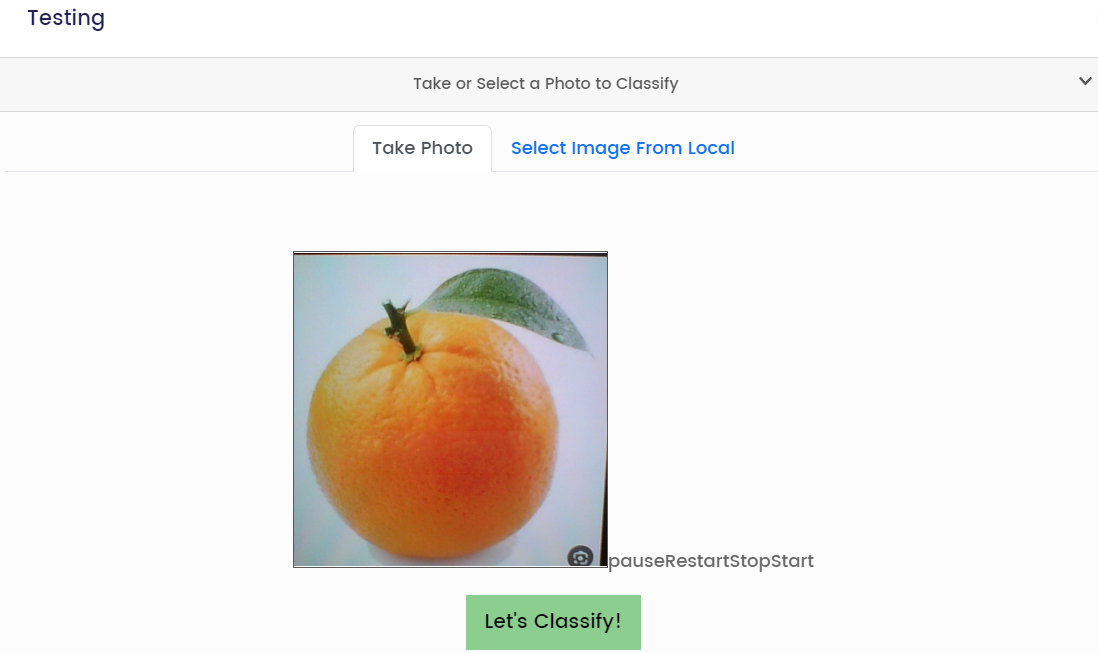
\includegraphics[width=\linewidth]{Chapters/Chapter_7/images/quality_check.png}
    \subcaption{Quality Check}
  \end{minipage}

  \vspace{0.5cm} % Adjust the vertical space between the images

  \begin{minipage}[b]{0.6\linewidth}
    \centering
    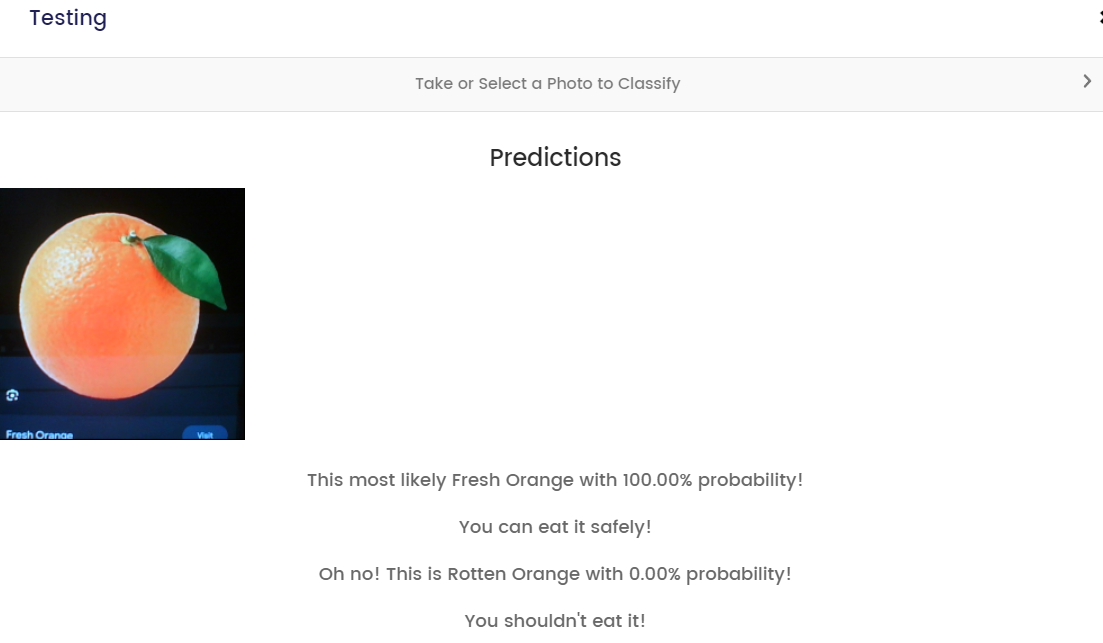
\includegraphics[width=\linewidth]{Chapters/Chapter_7/images/quality_check_result.png}
    \subcaption{Quality Check results}
  \end{minipage}
  
  \caption{Model Output}
  
  \label{fig:figure7_2}
\end{figure}
\noindent {Whenever an user wants to check whether the quality of the product is good or bad he can check that using an ML model,after checking the model is giving output as fresh if the fruit is in good condition and if not then the model is giving output as rotten.\par}
\noindent{The first diagram Figure \ref{fig:figure7_2}(A) is used to show how we can show the product to our camera sensor and after clicking on the let's clearift button it gives the result shown in the second diagram Figure i.e.\ref{fig:figure7_2}(B)}







